\documentclass{standalone}
\usepackage{tikz}
\usetikzlibrary{patterns, positioning}


\begin{document}
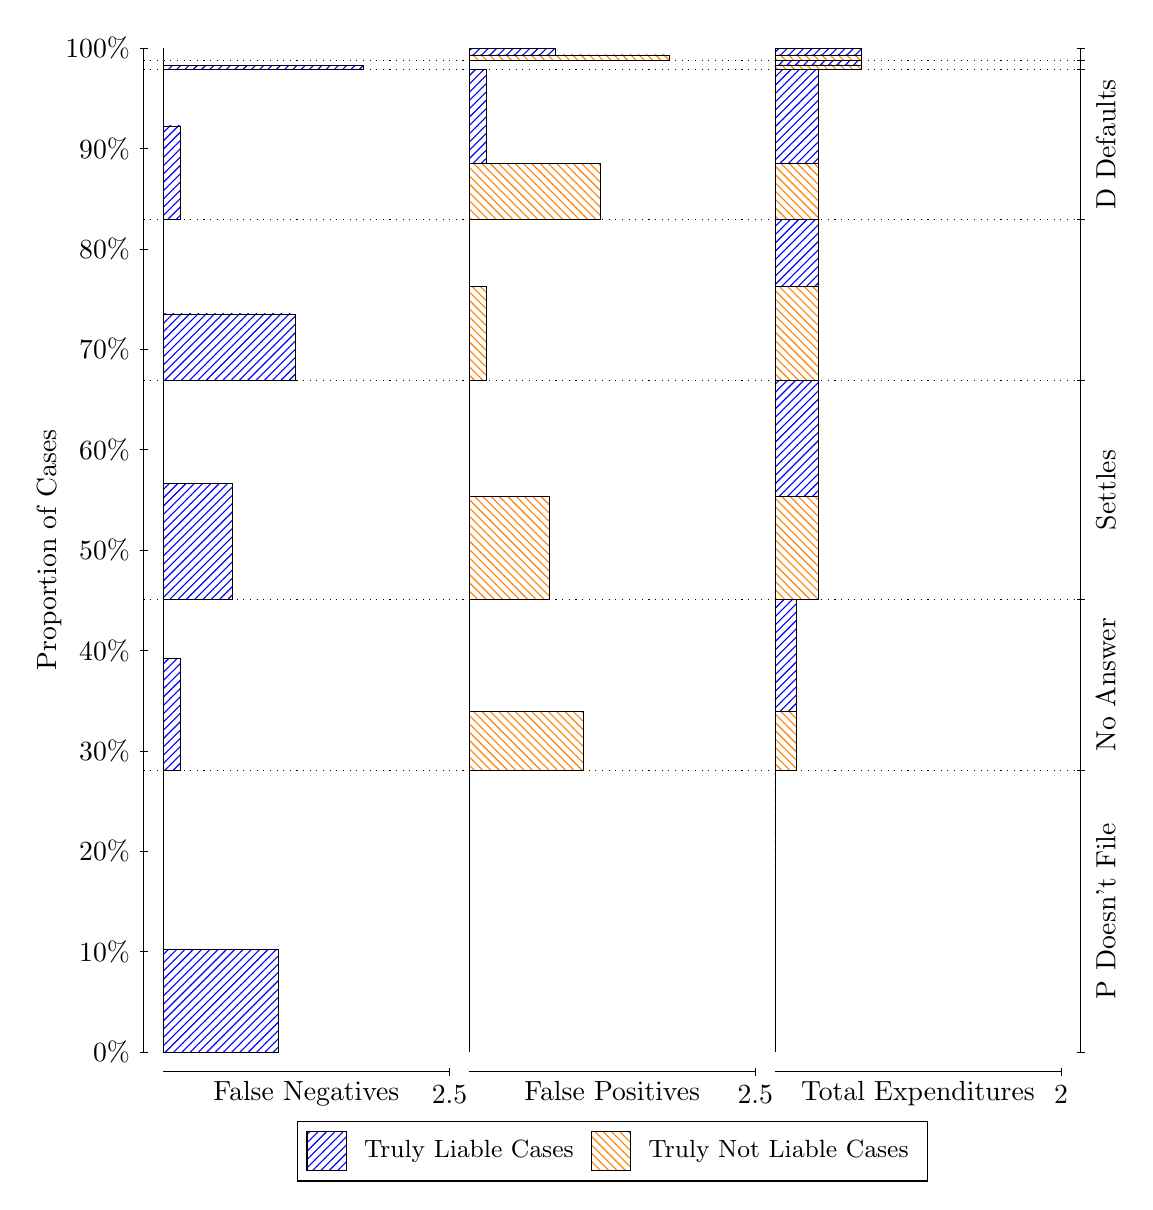
\begin{tikzpicture}
\draw[black, very thin] (1.5,1.75) -- (1.5,14.5);
\node[rotate=90, text=black, anchor=center] at (0.3, 8.125) {Proportion of Cases};
\draw[black, very thin] (1.45,1.75) -- (1.55,1.75);
\node[text=black, anchor=east] at (1.45, 1.75) {0\%};
\draw[black, very thin] (1.45,3.025) -- (1.55,3.025);
\node[text=black, anchor=east] at (1.45, 3.025) {10\%};
\draw[black, very thin] (1.45,4.3) -- (1.55,4.3);
\node[text=black, anchor=east] at (1.45, 4.3) {20\%};
\draw[black, very thin] (1.45,5.575) -- (1.55,5.575);
\node[text=black, anchor=east] at (1.45, 5.575) {30\%};
\draw[black, very thin] (1.45,6.85) -- (1.55,6.85);
\node[text=black, anchor=east] at (1.45, 6.85) {40\%};
\draw[black, very thin] (1.45,8.125) -- (1.55,8.125);
\node[text=black, anchor=east] at (1.45, 8.125) {50\%};
\draw[black, very thin] (1.45,9.4) -- (1.55,9.4);
\node[text=black, anchor=east] at (1.45, 9.4) {60\%};
\draw[black, very thin] (1.45,10.675) -- (1.55,10.675);
\node[text=black, anchor=east] at (1.45, 10.675) {70\%};
\draw[black, very thin] (1.45,11.95) -- (1.55,11.95);
\node[text=black, anchor=east] at (1.45, 11.95) {80\%};
\draw[black, very thin] (1.45,13.225) -- (1.55,13.225);
\node[text=black, anchor=east] at (1.45, 13.225) {90\%};
\draw[black, very thin] (1.45,14.5) -- (1.55,14.5);
\node[text=black, anchor=east] at (1.45, 14.5) {100\%};

\draw[black, very thin] (13.4,1.75) -- (13.4,14.5);
\draw[black, very thin] (13.35,1.75) -- (13.45,1.75);
\node[anchor=west] at (13.35, 1.75) {};
\draw[black, very thin] (13.35,5.3283) -- (13.45,5.3283);
\node[anchor=west] at (13.35, 5.3283) {};
\draw[black, very thin] (13.35,7.4989) -- (13.45,7.4989);
\node[anchor=west] at (13.35, 7.4989) {};
\draw[black, very thin] (13.35,10.276) -- (13.45,10.276);
\node[anchor=west] at (13.35, 10.276) {};
\draw[black, very thin] (13.35,12.324) -- (13.45,12.324);
\node[anchor=west] at (13.35, 12.324) {};
\draw[black, very thin] (13.35,14.225) -- (13.45,14.225);
\node[anchor=west] at (13.35, 14.225) {};
\draw[black, very thin] (13.35,14.342) -- (13.45,14.342);
\node[anchor=west] at (13.35, 14.342) {};
\draw[black, very thin] (13.35,14.5) -- (13.45,14.5);
\node[anchor=west] at (13.35, 14.5) {};

\draw[black, very thin, pattern color=blue, pattern=north east lines] (1.75,1.75) rectangle (3.2033,3.0543);
\draw[black, very thin, pattern color=orange, pattern=north west lines] (1.75,3.0543) rectangle (1.75,5.3283);
\draw[black, very thin, pattern color=blue, pattern=north east lines] (1.75,5.3283) rectangle (1.968,6.747);
\draw[black, very thin, pattern color=orange, pattern=north west lines] (1.75,6.747) rectangle (1.75,7.4989);
\draw[black, very thin, pattern color=blue, pattern=north east lines] (1.75,7.4989) rectangle (2.622,8.9695);
\draw[black, very thin, pattern color=orange, pattern=north west lines] (1.75,8.9695) rectangle (1.75,10.276);
\draw[black, very thin, pattern color=blue, pattern=north east lines] (1.75,10.276) rectangle (3.4213,11.125);
\draw[black, very thin, pattern color=orange, pattern=north west lines] (1.75,11.125) rectangle (1.75,12.324);
\draw[black, very thin, pattern color=blue, pattern=north east lines] (1.75,12.324) rectangle (1.968,13.511);
\draw[black, very thin, pattern color=orange, pattern=north west lines] (1.75,13.511) rectangle (1.75,14.225);
\draw[black, very thin, pattern color=blue, pattern=north east lines] (1.75,14.225) rectangle (4.2933,14.281);
\draw[black, very thin, pattern color=orange, pattern=north west lines] (1.75,14.281) rectangle (1.75,14.342);
\draw[black, very thin, pattern color=orange, pattern=north west lines] (1.75,14.342) rectangle (1.75,14.412);
\draw[black, very thin, pattern color=blue, pattern=north east lines] (1.75,14.412) rectangle (1.75,14.5);
\draw[black, very thin, pattern color=orange, pattern=north west lines] (5.6333,1.75) rectangle (5.6333,4.024);
\draw[black, very thin, pattern color=blue, pattern=north east lines] (5.6333,4.024) rectangle (5.6333,5.3283);
\draw[black, very thin, pattern color=orange, pattern=north west lines] (5.6333,5.3283) rectangle (7.0867,6.0801);
\draw[black, very thin, pattern color=blue, pattern=north east lines] (5.6333,6.0801) rectangle (5.6333,7.4989);
\draw[black, very thin, pattern color=orange, pattern=north west lines] (5.6333,7.4989) rectangle (6.6507,8.8054);
\draw[black, very thin, pattern color=blue, pattern=north east lines] (5.6333,8.8054) rectangle (5.6333,10.276);
\draw[black, very thin, pattern color=orange, pattern=north west lines] (5.6333,10.276) rectangle (5.8513,11.474);
\draw[black, very thin, pattern color=blue, pattern=north east lines] (5.6333,11.474) rectangle (5.6333,12.324);
\draw[black, very thin, pattern color=orange, pattern=north west lines] (5.6333,12.324) rectangle (7.3047,13.037);
\draw[black, very thin, pattern color=blue, pattern=north east lines] (5.6333,13.037) rectangle (5.8513,14.225);
\draw[black, very thin, pattern color=orange, pattern=north west lines] (5.6333,14.225) rectangle (5.6333,14.286);
\draw[black, very thin, pattern color=blue, pattern=north east lines] (5.6333,14.286) rectangle (5.6333,14.342);
\draw[black, very thin, pattern color=orange, pattern=north west lines] (5.6333,14.342) rectangle (8.1767,14.412);
\draw[black, very thin, pattern color=blue, pattern=north east lines] (5.6333,14.412) rectangle (6.7233,14.5);
\draw[black, very thin, pattern color=orange, pattern=north west lines] (9.5167,1.75) rectangle (9.5167,4.024);
\draw[black, very thin, pattern color=blue, pattern=north east lines] (9.5167,4.024) rectangle (9.5167,5.3283);
\draw[black, very thin, pattern color=orange, pattern=north west lines] (9.5167,5.3283) rectangle (9.7892,6.0801);
\draw[black, very thin, pattern color=blue, pattern=north east lines] (9.5167,6.0801) rectangle (9.7892,7.4989);
\draw[black, very thin, pattern color=orange, pattern=north west lines] (9.5167,7.4989) rectangle (10.062,8.8054);
\draw[black, very thin, pattern color=blue, pattern=north east lines] (9.5167,8.8054) rectangle (10.062,10.276);
\draw[black, very thin, pattern color=orange, pattern=north west lines] (9.5167,10.276) rectangle (10.062,11.474);
\draw[black, very thin, pattern color=blue, pattern=north east lines] (9.5167,11.474) rectangle (10.062,12.324);
\draw[black, very thin, pattern color=orange, pattern=north west lines] (9.5167,12.324) rectangle (10.062,13.037);
\draw[black, very thin, pattern color=blue, pattern=north east lines] (9.5167,13.037) rectangle (10.062,14.225);
\draw[black, very thin, pattern color=orange, pattern=north west lines] (9.5167,14.225) rectangle (10.607,14.286);
\draw[black, very thin, pattern color=blue, pattern=north east lines] (9.5167,14.286) rectangle (10.607,14.342);
\draw[black, very thin, pattern color=orange, pattern=north west lines] (9.5167,14.342) rectangle (10.607,14.412);
\draw[black, very thin, pattern color=blue, pattern=north east lines] (9.5167,14.412) rectangle (10.607,14.5);
\draw[black, dotted] (1.5,5.3283) -- (13.4,5.3283);
\draw[black, dotted] (1.5,7.4989) -- (13.4,7.4989);
\draw[black, dotted] (1.5,10.276) -- (13.4,10.276);
\draw[black, dotted] (1.5,12.324) -- (13.4,12.324);
\draw[black, dotted] (1.5,14.225) -- (13.4,14.225);
\draw[black, dotted] (1.5,14.342) -- (13.4,14.342);
\draw[black, very thin] (1.75,1.5) -- (5.3833,1.5);
\node[text=black, anchor=north] at (3.5667, 1.5) {False Negatives};
\draw[black, very thin] (5.3833,1.45) -- (5.3833,1.55);
\node[text=black, anchor=north] at (5.3833, 1.45) {2.5};

\draw[black, very thin] (5.6333,1.5) -- (9.2667,1.5);
\node[text=black, anchor=north] at (7.45, 1.5) {False Positives};
\draw[black, very thin] (9.2667,1.45) -- (9.2667,1.55);
\node[text=black, anchor=north] at (9.2667, 1.45) {2.5};

\draw[black, very thin] (9.5167,1.5) -- (13.15,1.5);
\node[text=black, anchor=north] at (11.333, 1.5) {Total Expenditures};
\draw[black, very thin] (13.15,1.45) -- (13.15,1.55);
\node[text=black, anchor=north] at (13.15, 1.45) {2};

\node[text=black, centered, rotate=90] at (13.72, 3.5391) {P Doesn't File};
\node[text=black, centered, rotate=90] at (13.72, 6.4136) {No Answer};
\node[text=black, centered, rotate=90] at (13.72, 8.8875) {Settles};

\node[text=black, centered, rotate=90] at (13.72, 13.274) {D Defaults};



\draw (7.449999999999999,1.5) node[draw=none] (baseCoordinate) {};
\begin{scope}[align=center]
        \matrix[scale=0.5, draw=black, below=0.5cm of baseCoordinate, nodes={draw}, column sep=0.1cm]{
            \node[rectangle, draw, minimum width=0.5cm, minimum height=0.5cm, pattern color=blue, pattern=north east lines] {}; &
            \node[draw=none, font=\small, text=black] (B) {Truly Liable Cases}; &
            \node[rectangle, draw, minimum width=0.5cm, minimum height=0.5cm, pattern color=orange, pattern=north west lines] {}; &
            \node[draw=none, font=\small, text=black] (B) {Truly Not Liable Cases}; \\
            };
\end{scope}

\end{tikzpicture}
\end{document}